%\documentclass[11pt]{amsproc}
%\documentclass[11pt]{article}
\documentclass[11pt]{article}
%\usepackage{setspace}
%\usepackage{fancyhdr}
\usepackage{fullpage}
\usepackage{graphicx}
\usepackage{amssymb}
%\usepackage{accents}
\usepackage{amsfonts}
\usepackage{amsthm}
\usepackage{amsmath}
\usepackage{eucal}
\usepackage{xypic}
\usepackage{pdfsync}
\usepackage{hyperref}
\usepackage{enumerate}



%%\setrightmargin{1in}
%\setallmargins{1in}

% Titlerule is a FAT ruler
\newcommand{\titlerule}{\rule{\linewidth}{1.5mm}}
% For comments in the draft - work in progress
\newcommand{\betainsert}[2]{\fbox{#1}\marginnote{\textsf{#2}}}

% Notes in the margin are nicer this way. HaHa
\newcommand{\marginnote}[1]{\marginpar{\scriptsize\raggedright #1}}



\def\bd{\partial}
\def\ra{\rightarrow}
\def\lra{\longrightarrow}
\def\Z{{\mathbb Z}}
\def\N{{\mathbb N}}
\def\R{{\mathbb R}}
\def\Q{{\mathbb Q}}
\def\C{{\mathbb C}}
\def\P{{\mathbb P}}
\def\K{{\mathbb K}}
\def\w{\mathcal{W}(E)}
\def\A{\mathcal{A}}
\def\B{\mathcal{B}}
\def\M{\mathcal{M}}
\def\N{\mathcal{N}}
\def\p{\partial}

\newcommand*{\longhookrightarrow}{\ensuremath{\lhook\joinrel\relbar\joinrel\rightarrow}}

\newtheorem{lem}{Lemma}
\newtheorem{prop}{Proposition}
\newtheorem{thm}{Theorem}
\newtheorem{cor}{Corollary}
\newtheorem{conj}{Conjecture}
\newtheorem{defn}{Definition}
\newtheorem{claim}{Claim}
\newtheorem{ques}{Question}
\newtheorem{rem}{Remark}

\theoremstyle{remark}
\newtheorem*{prob}{Problem}
\newtheorem{ex}{Example}
\def\T{\mathbb{T}}

\begin{document}
\begin{center}
    \begin{Large} {\bf Math 540 Homework 7}\\
    \end{Large}
    Haosen Wu  / Thur, Spet. 27, 2018
\end{center}
%\vspace{10mm}

\subsection*{1}
    Indeed we are proving the diagram below commutes:
    \[
    \xymatrix{
    & \tilde{X}/F \ar[d]^{\theta}  \ar[r]^{\rho(-)} & \Tilde{X}/F' \ar[d]^{\theta} &  \\
    & \tilde{X'}/F  \ar[r]^{\rho'(-)} & \Tilde{X'}/F' &
    }
    \]
    (Psychologically we distiguish $F,F'$ but $F=F'$ in fact.)
    
    The isomorphism of covering $\varphi: \tilde{X}\rightarrow \tilde{X'}$, combine with path lifting property (asserts the uniqueness), tells us that the lifting of path $\alpha$ whose $[\alpha] \in \pi_1(X;x_0)$ induces identical monodromy antihomomorphism $\rho(-)$ and $\rho'(-)$. But then (letting $x_0\in F$) $\rho([\alpha])\circ \theta(x_0)$ is sending $x_0$ first to some $y_0\in F$, then to $z'_0\in F'$; $\theta \circ \rho ' ([\alpha])$ is sending $x_0$ first to some $w'_0\in F'$, then to $z'_0\in F'$, since $w'_0=\rho([\alpha])(x_0),z'_0=\rho([\alpha])(y_0)$ as well $\rho([\alpha])$ preserves the sending. Therefore $ \theta \circ \rho ' ([\alpha]) = \rho([\alpha])\circ \theta(x_0)$, the diagram commutes, which is equivalent to say $\rho ([\alpha])=\theta \circ \rho ' ([\alpha]) \circ \theta^{-1}$.
    
    (Abuse of notation here)  
    
    Conversely, if diagram commutes, map $\rho(-)$ can construct map from covering $\tilde{X}$ to covering $\tilde{X'}$ by gluing up fibers, as ball around fiber provides natural local homeomorphism; Inverse of $\rho(-)$ provides inverse map from covering $\tilde{X'}$ to covering $\tilde{X}$. Then the map between coverings provides an  isomorphism.
    
    (The converse part has been proved in class, as realizing the same $\rho(-)$ for both coverings. Some abstract proof can be given as: identify elements in Bij(F) as group action elements in $S_n$, $n$ is cardinality of fiber, then result is immediate from elements in $S_n$ conjugates iff they have same cycle type. This proof is good but only when fiber is finite.) 
    
\subsection*{General Lemma for 2 and 3}
  \indent (For Connected Covering) We investigate $p_*(\pi(\tilde{X};\tilde{x_0})\in \pi(X;x_0)$
  
  (For All Covering) We follow the fashion in Problem 1,  which tells us $n$-sheet covering space is \textit{really} classified by equivalence classes of homomorphisms from $\pi_1(X;x_0)$ to $S_n$. 
\subsection*{2 & }
    
    By general lemma (with $Id_F$), Group $\Z\times\Z$ has following homomorphisms to $S_3$: As $\pi_1(S^1\times S^1;x_0)=\Z\times\Z$ is abelian,   $\varphi(\alpha)\varphi(\beta)=\varphi(\alpha\beta)=\varphi(\beta\alpha)=\varphi(\beta)\varphi(\alpha)$, and the image of $\Z\times\Z$ has also to be abelian, as in figure 7-2 we have $18$ homomorphisms, or coverings ($Id_F$=fixed isomorphic).
    
    \begin{figure}[h!]
    \centering
    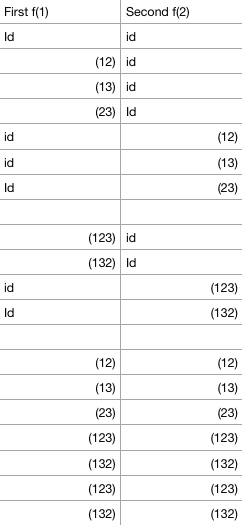
\includegraphics[scale=0.5]{7-2.png}
    \caption{7-2}
    \end{figure}
     
    When not fixing F, we are talking about: by general lemma the conjugacy class of homomorphisms induced by monodromy tells us the not-fixing-F homomorphisms. We are finding them by looking at \textit{equivalence class of cycles} that commutes. If $\varphi(\alpha)$ map to identity, we can have mapped to identity, 2-cycle and 3-cycle; If $\varphi(\alpha)$ map to 2-cycle, we can have mapped to identity, 2-cycle; If $\varphi(\alpha)$ map to 3-cycle, we can have mapped to identity, itself and another 3-cycle. Therefore in total we have 8 conjugate homomorphisms, or coverings. 
    
\subsection*{ & 3}    
    group $\langle a,b; a^2=b^2 \rangle$ has following homomorphisms to $S_3$:   ${\varphi(\alpha)}^2=\varphi(\alpha^2)=\varphi(\beta^2)=\varphi(\beta)^2$, and the image of $\langle a,b; a^2=b^2 \rangle$ has also to be \textit{square-identical}, as in figure 7-3 we have $18$ homomorphisms (surprisingly same), or coverings ($Id_F$=fixed isomorphic).
    
    \begin{figure}[h!]
    \centering
    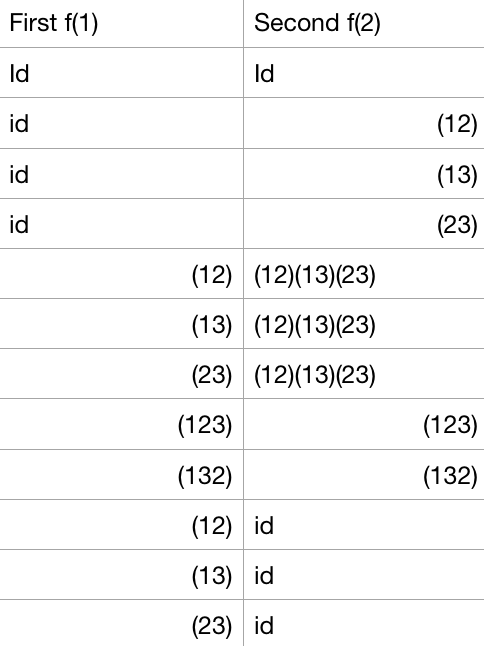
\includegraphics[scale=0.5]{7-3_update.png}
    \caption{7-3}
    \end{figure}
    
    When not fixing F, we are talking about: by general lemma the conjugacy class of homomorphisms induced by monodromy tells us the not-fixing-F homomorphisms. We are finding them by looking at \textit{equivalence class of cycles} that are also \textit{square-identical}. If $\varphi(\alpha)$ map to identity, we can have mapped to identity, 2-cycle; If $\varphi(\alpha)$ map to 2-cycle, we can have mapped to identity, 2-cycle; If $\varphi(\alpha)$ map to 3-cycle, we can have mapped to identity, itself. Therefore in total we have 6 homomorphisms, or coverings. 
    
    
\subsection*{ & }     
    Thus we completed 3-sheets covering classification for 2 & 3.
\subsection*{4}
    Only need lift (on $\tilde{\alpha(0)}=\tilde{x_0}$, then by unique path lifting, and our $F=\Z$ is infinite: 
    \\lift $\rho{[\alpha]}(\tilde{x_0})=$One-level-up $x_0$. (Shift $F=\Z$ with One-level-up) 
    \\lift $\rho{[\beta]}(\tilde{x_0})=$Two-level-up $x_0$. (Shift $F=\Z$ with Two-level-up) 
    \\lift $\rho{[\gamma]}(\tilde{x_0})=$One-level-down $x_0$. (Shift $F=\Z$  with One-level-down) \\Haha, Nice parking lot! 

\end{document}
\frac{\pi}{}